% compile if you want a poster in portrait orientation

\documentclass[25pt, a0paper,portrait]{tikzposter} %orientation options: portrait, landscape
\usepackage[utf8]{inputenc}

\title{Thesis Title}
\author{[Full Name] ([Registration Number]) \\
Supervisor: Dr. Fahmizal}
\date{November 2021}
\institute{Department of Electrical Engineering and Informatics, Vocational College, UGM}

\usepackage[backend=biber, style=numeric, sorting=none, locallabelwidth]{biblatex}
\bibliography{ref}

\usetheme{Rays} % Options: Default, Simple, Basic, Rays, Wave, Envelope, Board, Autumn, Desert

\graphicspath{Images/}

%import necessary packages
\usepackage{blindtext}
\usepackage{graphicx}
\usepackage{caption}
\usepackage{subcaption}
\usepackage{comment}
\usepackage{amsmath,amssymb}

\begin{document}

\maketitle

\node[anchor=west, xshift = -1 cm ] at (TP@title.west) {
\includegraphics[width=10cm]{Images/logo-ugm.png}}; %left logo, comment out if unnecessary
\node[anchor=east, xshift = 1 cm] at (TP@title.east) {
\includegraphics[width=10cm]{Images/logo otomasi ugm.png}}; %right logo, comment out if unnecessary

\block{Abstract}
{
  \blindtext
}


\begin{columns}

    \column{0.6}%set width of first column

    \block{1. Introduction}{
        \blindtext[2]
        \begin{tikzfigure}
            
\includegraphics[scale=0.8]{Images/im1.png}
        \end{tikzfigure}
    
    }

    
    \block{3. Key Results}{
        \blindenumerate[3]
        \blindtext
        \blindenumerate[2]
    }

    
    \block{5. Future Work}{
        \blindtext
        \blindenumerate[2]    
    }
    

    
    \column{0.4}%set width of second column

    \block{2. Method}{
        \blindenumerate[7]
    }

    \block{4. Examples}
    {
        \blindtext
        \begin{equation}
            \int \Vec{F}.d\Vec{q}=-U
        \end{equation}
        \begin{tikzfigure}
            
\includegraphics[scale=0.8]{Images/im2.png}
        \end{tikzfigure}
    }

    \block{6. Plots}{
        \begin{tikzfigure}
            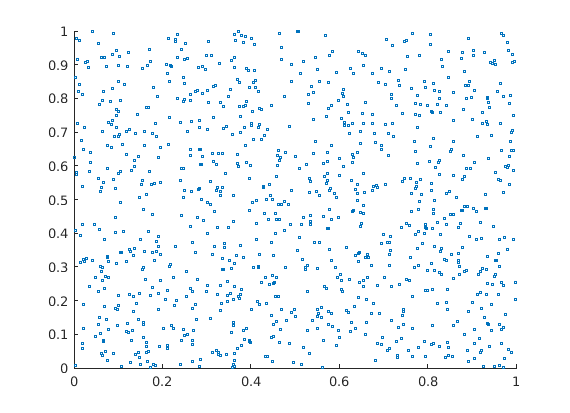
\includegraphics[scale=0.8]{Images/plot1.png}
        \end{tikzfigure}
        \begin{tikzfigure}
            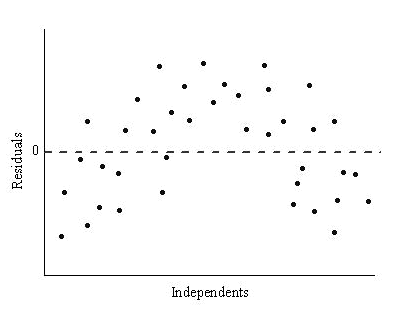
\includegraphics[scale=1.0]{Images/plot2.png}
        \end{tikzfigure}
    }
        

    %if necessary, add more columns, adjusting the widths
    %more columns may be necessary in landscape mode
    
\end{columns}

\block{References}{
    \nocite{*}
    \begin{minipage}{\linewidth}
        \begin{center}\mbox{}\vspace{-\baselineskip}
        \printbibliography[heading=none]
    \end{center}
    \end{minipage}
    }

\end{document}
